\documentclass[
  bibliography=totoc,     % Literatur im Inhaltsverzeichnis
  captions=tableheading,  % Tabellenüberschriften
  titlepage=firstiscover, % Titelseite ist Deckblatt
]{scrartcl}

% Paket float verbessern
\usepackage{scrhack}

% Warnung, falls nochmal kompiliert werden muss
\usepackage[aux]{rerunfilecheck}

% unverzichtbare Mathe-Befehle
\usepackage{amsmath}
% viele Mathe-Symbole
\usepackage{amssymb}
% Erweiterungen für amsmath
\usepackage{mathtools}

% Fonteinstellungen
\usepackage{fontspec}
% Latin Modern Fonts werden automatisch geladen
% Alternativ:
%\setromanfont{Libertinus Serif}
%\setsansfont{Libertinus Sans}
%\setmonofont{Libertinus Mono}
\recalctypearea % Wenn man andere Schriftarten gesetzt hat,
% sollte man das Seiten-Layout neu berechnen lassen

% deutsche Spracheinstellungen
\usepackage{polyglossia}
\setmainlanguage{german}


\usepackage[
  math-style=ISO,    % ┐
  bold-style=ISO,    % │
  sans-style=italic, % │ ISO-Standard folgen
  nabla=upright,     % │
  partial=upright,   % ┘
  warnings-off={           % ┐
    mathtools-colon,       % │ unnötige Warnungen ausschalten
    mathtools-overbracket, % │
},                       % ┘
]{unicode-math}

% traditionelle Fonts für Mathematik
\setmathfont{Latin Modern Math}
% Alternativ:
%\setmathfont{Libertinus Math}

\setmathfont{XITS Math}[range={scr, bfscr}]
\setmathfont{XITS Math}[range={cal, bfcal}, StylisticSet=1]

% Zahlen und Einheiten
\usepackage[
locale=DE,                   % deutsche Einstellungen
separate-uncertainty=true,   % immer Fehler mit \pm
per-mode=symbol-or-fraction, % / in inline math, fraction in display math
]{siunitx}

% chemische Formeln
\usepackage[
version=4,
math-greek=default, % ┐ mit unicode-math zusammenarbeiten
text-greek=default, % ┘
]{mhchem}

% richtige Anführungszeichen
\usepackage[autostyle]{csquotes}

% schöne Brüche im Text
\usepackage{xfrac}

% Standardplatzierung für Floats einstellen
\usepackage{float}
\floatplacement{figure}{htbp}
\floatplacement{table}{htbp}

% Floats innerhalb einer Section halten
\usepackage[
section, % Floats innerhalb der Section halten
below,   % unterhalb der Section aber auf der selben Seite ist ok
]{placeins}

% Seite drehen für breite Tabellen: landscape Umgebung
\usepackage{pdflscape}

% Captions schöner machen.
\usepackage[
  labelfont=bf,        % Tabelle x: Abbildung y: ist jetzt fett
  font=small,          % Schrift etwas kleiner als Dokument
  width=0.9\textwidth, % maximale Breite einer Caption schmaler
]{caption}
% subfigure, subtable, subref
\usepackage{subcaption}

% Grafiken können eingebunden werden
\usepackage{graphicx}
% größere Variation von Dateinamen möglich
\usepackage{grffile}

% schöne Tabellen
\usepackage{booktabs}

% Verbesserungen am Schriftbild
\usepackage{microtype}

% Literaturverzeichnis
\usepackage[style=alphabetic,]{biblatex}
% Quellendatenbank
\addbibresource{lit.bib}
\addbibresource{programme.bib}

% Hyperlinks im Dokument
\usepackage[
  unicode,        % Unicode in PDF-Attributen erlauben
  pdfusetitle,    % Titel, Autoren und Datum als PDF-Attribute
  pdfcreator={},  % ┐ PDF-Attribute säubern
  pdfproducer={}, % ┘
]{hyperref}
% erweiterte Bookmarks im PDF
\usepackage{bookmark}

% Trennung von Wörtern mit Strichen
\usepackage[shortcuts]{extdash}

\title{SMD: Blatt 1}
\author{
  Sophie Bork
  \texorpdfstring{
    \\
    \href{mailto:sophie.bork@udo.edu}{sophie.bork@udo.edu}
  }{}
  \texorpdfstring{\and}{, }
  Michael Windau
  \texorpdfstring{
    \\
    \href{mailto:michael.windau@udo.edu}{michael.windau@udo.edu}
  }{}
  \texorpdfstring{\and}{, }
  Simon Schulte
  \texorpdfstring{
    \\
    \href{mailto:simon.schulte@udo.edu}{simon.schulte@udo.edu}
  }{}
}
\publishers{TU Dortmund – Fakultät Physik}


\begin{document}

\maketitle
\thispagestyle{empty}
\newpage
\setcounter{page}{1}
\section{. Aufgabe}
\noindent
In den Abbildungen \ref{fig:1}, \ref{fig:2} und \ref{fig:3} sind beide Funktionen
zusammen für Werte zwischen $\num{e-6}$ und $\num{e6}$ bzw. einzeln in dem
jeweiligen kritischen Bereich dargestellt.
\begin{figure}[H]
  \centering
  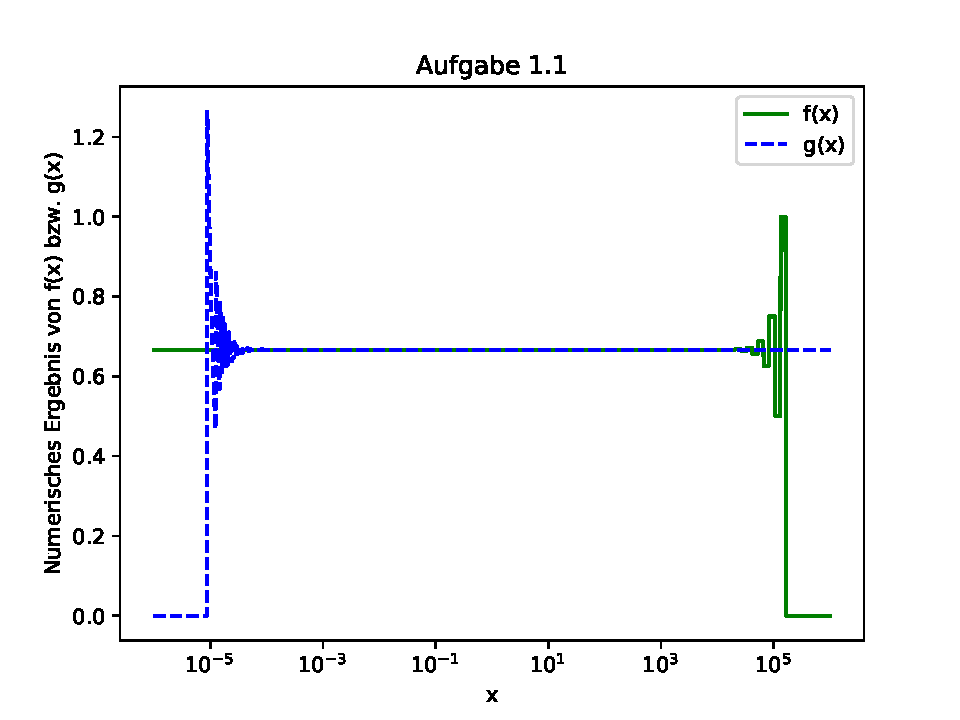
\includegraphics[width=\textwidth]{aufgabe11.pdf}
  \caption{Beide Funktionen.}
  \label{fig:1}
\end{figure}
\begin{figure}[H]
  \centering
  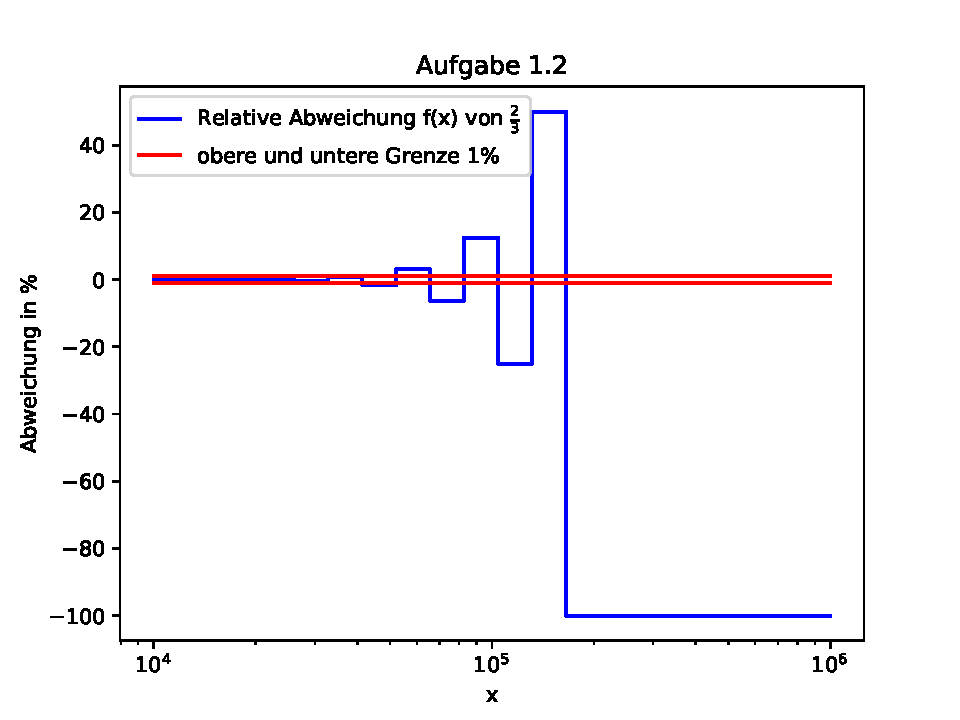
\includegraphics[width=0.8\textwidth]{aufgabe12.pdf}
  \caption{f(x).}
  \label{fig:2}
\end{figure}
\begin{figure}[H]
  \centering
  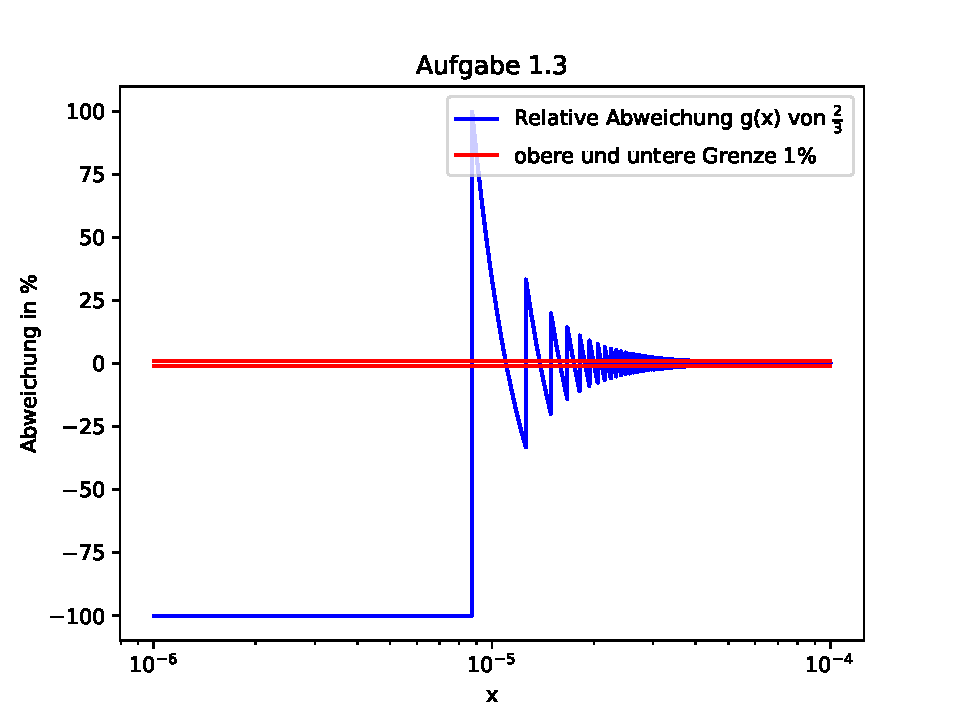
\includegraphics[width=0.8\textwidth]{aufgabe13.pdf}
  \caption{g(x).}
  \label{fig:3}
\end{figure}
\clearpage
\noindent
Das numerische Ergebnis von f(x) weicht bis etwa $\num{4e4}$ um weniger als $\SI{1}{\percent}$
von $\frac{2}{3}$ ab und ist ab $\num{2e5}$ gleich Null.
Das numerische Ergebnis von g(x) weicht ab etwa $\num{4e-5}$ um weniger als $\SI{1}{\percent}$
von $\frac{2}{3}$ ab und ist bis $\num{8e-6}$ gleich Null.

\section{. Aufgabe}
\noindent
a) Die Gleichung ist nicht überall stabil. Bei 0 und bei Vielfachen von $\pi$
ist die Gleichung instabil, da dort durch eine sehr kleine Zahl geteilt wird.\\

\noindent
b) Die Instabilität lässt sich durch eine Umformung der Funktion zu
\begin{equation*}
  \frac{\mathup{d}\sigma}{\mathup{d}\Omega}= \frac{\alpha^2}{s} \left(\frac{(\sin(\theta)^2+2)\gamma^2}{\gamma^2 \sin(\theta)^2 + \cos(\theta)^2}\right)
\end{equation*}
beheben.\\

\noindent
c) In Abbildung \ref{fig:4} ist der Wirkungsquerschnitt für die ursprüngliche Funktion
und für die umgeformte Funktion zwischen $0$ und $2\pi$ dargestellt.
Dabei ist noch keine Instabilität zu erkennen. In Abbildung \ref{fig:5}
sind beide Funktionen in der Nähe von $\pi$ dargestellt. Die Umformung hat also
das Problem behoben.
\begin{figure}[H]
  \centering
  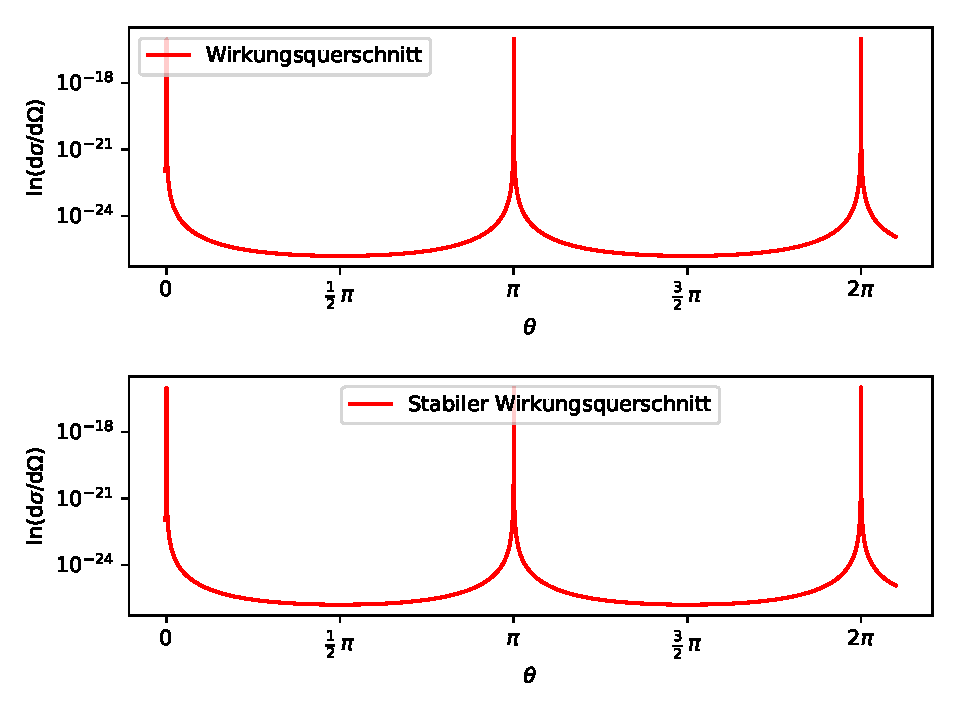
\includegraphics[width=0.8\textwidth]{wirkungsquerschnitt1.pdf}
  \caption{Beide Formen zwischen $0$ und $2 \pi$.}
  \label{fig:4}
\end{figure}
\begin{figure}[H]
  \centering
  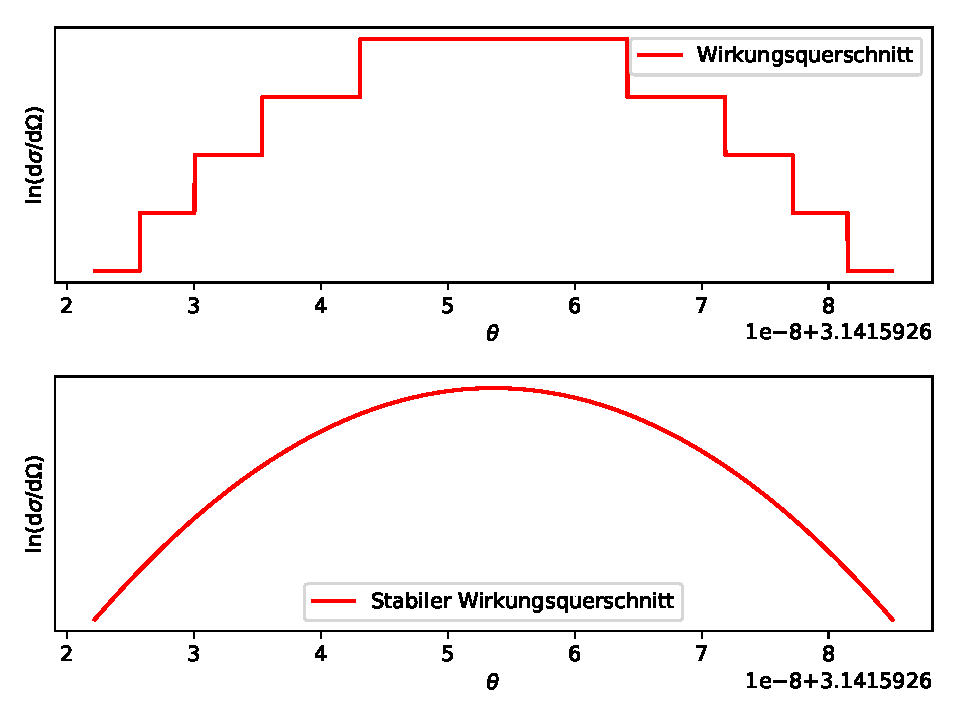
\includegraphics[width=0.7\textwidth]{wirkungsquerschnitt2.pdf}
  \caption{Beim näheren Betrachten der kritischen Bereiche sieht man, dass die Umformung das Problem behoben hat.}
  \label{fig:5}
\end{figure}

\noindent
d) $K = |\theta  \frac{2 \sin(\theta)\cos(\theta)(-3\beta^2+1)}{(2+\sin(\theta)^2)(1 - \beta^2  \cos(\theta)^2)^2}|$\\

\noindent
e) Der Verlauf der Konditionszahl ist in Abbildung \ref{fig:6} dargestellt.
Für $K \geq 1$ ist das Problem schlecht konditioniert.
\begin{figure}[H]
  \centering
  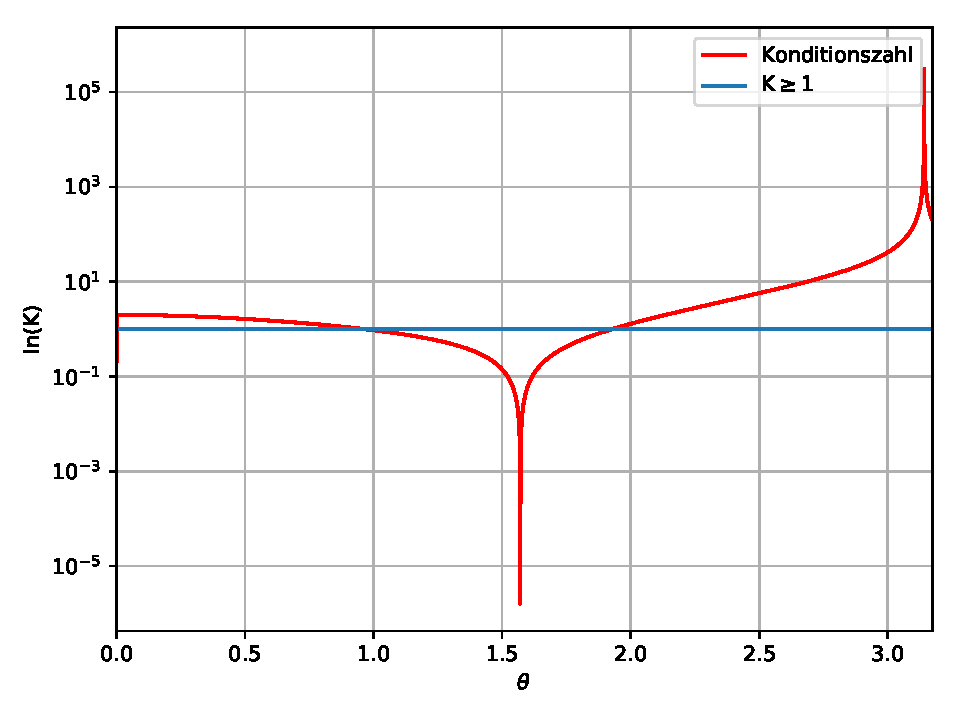
\includegraphics[width=0.7\textwidth]{konditionierung.pdf}
  \caption{Verlauf der Konditionszahl für das ursprüngliche Problem.}
  \label{fig:6}
\end{figure}

\section{. Aufgabe}
\noindent
Zuerst muss der Normierungsfaktor $N$ bestimmt werden.
Er ergibt sich aus der Bedingung:
\begin{equation*}
  \int_0^\infty \exp\left(-\frac{mv^2}{2k_\mathup{B}T}\right)\cdot4\pi v^2 \mathup{d}v = \frac{1}{N}
\end{equation*}
\noindent
\begin{equation*}
  N = \left(\frac{m}{2 \pi k_\mathup{B} T}\right)^\frac{3}{2}
\end{equation*}
Und damit:
\begin{equation*}
  f(v) = \left(\frac{m}{2 \pi k_\mathup{B} T}\right)^\frac{3}{2} \cdot \exp\left(-\frac{mv^2}{2k_\mathup{B}T}\right)\cdot4\pi v^2
\end{equation*}

\noindent
a) Für die Bestimmung der wahrscheinlichsten Geschwindigkeit $v_\mathup{m}$ wird das Maximum der Verteilung
berechnet. Mit der notwendigen Bedinung für Extrema ergibt sich:
\begin{equation*}
  v_\mathup{m} = \sqrt{\frac{2k_\mathup{B}T}{m}}
\end{equation*}
b)-e) /

\section{. Aufgabe}
\noindent
a) Für den Fall, dass die Summe der Würfelaugen 9 ergibt, gibt es 4 Möglichkeiten.
Jede von diesen hat eine Wahrscheinlichkeit von $\frac{1}{36}$:

$P(W_\text{rot}+W_\text{blau}=9) = \frac{4}{36} = \frac{1}{9}$\\

\noindent
b) Es gibt 10 Möglichkeiten eine Summe größer oder gleich 9 zu erhalten:

$P(W_\text{rot}+W_\text{blau} \geq 9) = \frac{10}{36} = \frac{5}{18}$\\

\noindent
c) Hier gibt es 2 Möglichkeiten:

$P(W_1=4, W_2=5) = \frac{2}{36} = \frac{1}{18}$\\

\noindent
d) $P(W_\text{rot}=4, W_\text{blau}=5) = \frac{1}{36}$\\

\noindent
e) $P(W_\text{rot}+W_\text{blau}=9|W_\text{rot}=4) = \frac{1}{6}$\\

\noindent
f) $P(W_\text{rot}+W_\text{blau} \geq 9|W_\text{rot}=4) = \frac{2}{6}$\\

\noindent
g) $P(W_\text{rot}=4, W_\text{blau}=5|W_\text{rot}=4) = \frac{1}{6}$

\end{document}
